\documentclass[article]{jss}

%%%%%%%%%%%%%%%%%%%%%%%%%%%%%%
%% declarations for jss.cls %%%%%%%%%%%%%%%%%%%%%%%%%%%%%%%%%%%%%%%%%%
%%%%%%%%%%%%%%%%%%%%%%%%%%%%%%

%% almost as usual
\author{Paul Deveau\\Institut Curie\\PSL Research University\\Univ. Paris-Sud\\INSERM U830\\INSERM U900\\Mines-ParisTech \And 
        Eric Bonnet\\Institut Curie\\PSL Research University\\INSERM U900\\Mines-ParisTech}
\title{Calculating Module Enrichment and Visualizing Data on Large-scale Molecular Maps with the R packages \pkg{ACSNMineR} and \pkg{RNaviCell}}

%% for pretty printing and a nice hypersummary also set:
\Plainauthor{Paul Deveau, Eric Bonnet} %% comma-separated
\Plaintitle{Calculating Module Enrichment and Visualizing Data on Large-scale Molecular Maps with the R packages ACSNMineR and RNaviCel} %% without formatting
\Shorttitle{Module Enrichment and Data Visualization with ACSNMineR and RNaviCell} %% a short title (if necessary)

%% an abstract and keywords
\Abstract{
  The abstract of the article.
}
\Keywords{keywords, comma-separated, not capitalized, \proglang{Java}}
\Plainkeywords{keywords, comma-separated, not capitalized, Java} %% without formatting
%% at least one keyword must be supplied

%% publication information
%% NOTE: Typically, this can be left commented and will be filled out by the technical editor
%% \Volume{50}
%% \Issue{9}
%% \Month{June}
%% \Year{2012}
%% \Submitdate{2012-06-04}
%% \Acceptdate{2012-06-04}

%% The address of (at least) one author should be given
%% in the following format:
\Address{
  Eric Bonnet\\
  Computational Systems Biology of Cancer\\
  Institut Curie\\
  26, rue d'Ulm\\
  75248 Paris, France\\
  E-mail: \email{eric.bonnet@curie.fr}\\
}
%% It is also possible to add a telephone and fax number
%% before the e-mail in the following format:
%% Telephone: +43/512/507-7103
%% Fax: +43/512/507-2851

%% for those who use Sweave please include the following line (with % symbols):
%% need no \usepackage{Sweave.sty}

%% end of declarations %%%%%%%%%%%%%%%%%%%%%%%%%%%%%%%%%%%%%%%%%%%%%%%


\begin{document}

%% include your article here, just as usual
%% Note that you should use the \pkg{}, \proglang{} and \code{} commands.

\section[Introduction]{Introduction}
Biological pathways and networks comprise sets of interactions or functional
relationships, occurring at the molecular level in living cells
\citep{adriaens2008public}.  A large body of knowledge on cellular biochemistry
is organized in publicly available repositories such as the KEGG database
\citep{kanehisa2011kegg}, Reactome \citep{croft2014reactome} and MINT
\citep{zanzoni2002mint}. All these biological databases facilitate a large
spectrum of analyses, improving our understanding of cellular systems. For
instance, it is a very common practice to cross the output of high-throughput
experiments, such as mRNA or protein expression levels, with curated biological
pathways in order to visualize changes, analyze their impact on a network and
formulate new hypotheses about biological processes. Many biologists and
computational biologists establish list of genes of interest (e.g. a list of
genes that are differentially expressed between two conditions, such as normal
vs disease) and then try to see if known biological pathways are enriched with
this list of genes. 

We have recently released the Atlas of Cancer Signalling Network (ACSN), a
web-based database which describes signaling and regulatory molecular processes
that occur in a healthy mammalian cell but that are frequently deregulated
during cancerogenesis \citep{kuperstein2013navicell}.  The ACSN atlas aims to
be a comprehensive description of cancer-related mechanisms retrieved from the
most recent literature. The web interface for ACSN is using the NaviCell
technology, a software framework dedicated to web-based visualization and
navigation for biological pathway maps \citep{kuperstein2013navicell}. This
environment is providing an easy navigation of maps through the use of the
Google Maps JavaScript library, a community interface with a web blog system,
and a comprehensive module for visualization and analysis of high-throughput
data \citep{bonnet2015navicell}.


In this article, we describe two software packages related to ACSN analysis and
data visualization for the popular R statistical enrironment \citep{mainRref,
vance2009data}. The package \pkg{ACSNMineR} is designed for the calculation of
gene enrichment and depletion in ACSN maps, while \pkg{RNaviCell} is dedicated
to data visualization on ACSN maps. Both packages are available on the
Comprehensive R Archive Network
(\url{https://cran.r-project.org/web/packages/ACSNMineR/} and
\url{https://cran.r-project.org/web/packages/RNaviCell/}), and on the GitHub
repository (\url{https://github.com/sysbio-curie/ACSNMineR} and
\url{https://github.com/sysbio-curie/RNaviCell}). For the remainder of this
article, we describe the organization of each package and illustrate their
capacities with several concrete examples demonstrating their capabilities. 

\section[Package organization]{Packages organization}

\subsection{ACSNMineR}
Currently, ACSN maps covers signaling pathways involved in DNA repair, cell
cycle, cell survival, cell death, epithelial-to-mesenchymal transition (EMT) and
cell motility. Each of these large-scale molecular map is decomposed in a number
of functional modules. The maps themselves are merged into a global ACSN map.
Thus the information included in ACSN is organized in three hierarchical levels:
a global map, five individual maps, and a total of 55 functional modules. Each
ACSN map covers hundreds of molecular players, biochemical reactions and causal
relationships between the molecular players and cellular phenotypes.  ACSN
represents a large-scale biochemical reaction network of 4,826 reactions
involving 2,371 proteins, and is continuously updated and expanded.  We have
included the three hierarchical levels in the \pkg{ACSNMineR} package, in order
to be able to calculate enrichments at all three levels. The calculations are
made by counting the number of occurences of gene symbols (HUGO gene names) from
a given list of genes of interest in all ACSN maps and modules. Table
\ref{tab:table1} is detailling the number of gene symbols contained in all the ACSN
maps.


\begin{table}[h!]
 \centering
  \caption{ACSN maps included in the \pkg{ACSNMineR} package. Map: map name, Total: total
  number of gene symbols (HUGO), Nb mod.: number of modules, Min: mimimum
  number of gene symbols in the modules, Max: maximum number of gene symbols in
  the modules, Mean: average number of gene sybols per module. N.B.: one gene
  symbol may be present in several modules of the map.}
  \label{tab:table1}
  \begin{tabular}{l|c|c|c|c|c}
    \hline
    Map & Total & Nb mod. & Min & Max & Mean\\
    \hline
  ACSN global & 2137 & 55 & 2 &625& 85\\
  Survival  &1065&46  &1 &434 &54\\
  Apoptosis & 668&44 & 1& 382& 33\\
  EMT \& Cell motility &620 &41  &1 &615 &43\\
  DNA repair &337&48  &1 &69  &19\\
  Cell cycle &119&45  &1 &27  &8\\
  \hline

  \end{tabular}

\end{table}


The statistical significance of the counts in the modules is assessed by using
either the Fisher exact test \citep{fisher1922interpretation,
fisher1934statistical} or the hypergeometric test, which are equivalent for this
purpose \citep{rivals2007enrichment}.

The current ACSN maps are included in the \pkg{ACSNMineR} package, as a list of character matrices.

\begin{verbatim}
> length(ACSN_maps)
[1] 6
> names(ACSN_maps)
[1] "Apoptosis"    "CellCycle"    "DNA_repair"   "EMT_motility" "ACSN_master" 
[6] "Survival"    
\end{verbatim}

For each matrix, rows represent a module, with the name of the module in the
first column, followed by a description of the module (optional), and then
followed by all the gene symbols of the module. The maps will be updated
according to every ACSN major release.

The main function of the \pkg{ACSNMineR} package is the \code{enrichment}
function, which is calculating over-representation or depletion of genes in the
ACSN maps and modules. We have included a small list of 12 Cell Cycle related
genes in the package, named \code{genes_test} that can be used to test the main
enrichment function and to get familiar with its different options.

\begin{verbatim}
> genes_test
 [1] "ATM"     "ATR"     "CHEK2"   "CREBBP"  "TFDP1"   "E2F1"    "EP300"  
 [8] "HDAC1"   "KAT2B"   "GTF2H1"  "GTF2H2"  "GTF2H2B"
\end{verbatim}

The example shown below is the simplest command that can be done to test a gene
list for over-representation on the six included ACSN maps. With the list of 12
genes mentionned above and a default p-value cutoff of $0.05$, we have a set of
36 maps or modules that are significantly enriched. The results are structured
as a data frame with nine columns displaying the module name, the module size,
the number of genes from the list in the module, the names of the genes that are
present in the module, the size of the reference universe, the number of genes
from the list that are present in the universe, the raw p-value, the p-value
corrected for multiple testing and the type of test performed. The module field
in the results data frame indicate the map name and the module name separated by
a column character. If a complete map is significantly enriched or depleted,
then only the map name is shown, without any module or column character. For
instance, the first line of the results object below concern the E2F1 module of
the Apoptosis map. 


\begin{verbatim}
> library(ACSNMineR)
> results <- enrichment(genes_test)
> dim(results)
[1] 36  9
> results[1,]
            module module_size nb_genes_in_module      genes_in_module
V12 Apoptosis:E2F1           5                  4 ATM E2F1 EP300 KAT2B
    universe_size nb_genes_in_universe      p.value p.value.corrected    test
V12          2133                   12 1.043478e-08       2.81739e-07 greater
\end{verbatim}


%    enrichment(Genes = NULL, maps = ACSNMineR::ACSN_maps,
%       correction_multitest = "BH", statistical_test = "fisher",
%       min_module_size = 5, universe = "map_defined", threshold = 0.05,
%       alternative = "greater")

The \code{enrichment} function can take up to eight arguments: the gene list (as
a character vector), the list of maps that will be used to calculate enrichment
or depletion, the type of statistical test (either the Fisher exact test or the
hypergeometric test), the module minimal size for which the calculations will be
done, the universe, the p-value threshold and the alternative ("greater" for
calculating over-representation, "less" for depletion and "both" for both
tests).

Only the gene list is mandatory to call the \code{enrichment} function, all the
other arguments have default values.  The \code{maps} argument can either be a
dataframe imported from a gmt file with the \code{format_from_gmt} function or
a list of dataframes generated by the same procedure. By default, the function
uses the ACSN maps previously described.  The correction for multiple testing
is set by default to false discovery rate (FDR), which is equivalent to
Benjamini \& Hochberg correction, but can be changed to any of the usual
correction methods (Bonferroni, Holm, Hochberg, Holm, or Benjamini \& Yekutieli
\citep{Benjamini2003FDR}), or even disabled .  The minimal module size
represents the smallest size value of a module that will be used to compute
enrichment or depletion. This is meant to remove results of low significance
for module of small size.  The universe in which the computation is made by
default is defined by all the gene symbols conatined in the maps. All the genes
that were given as input and that are not present on the maps will be
discarded. To keep all genes, the user can change the universe to \code{HUGO},
and in that case, the complete list of HUGO gene symbols will be used as the
reference ($>$ 39,000 genes). The threshold corresponds to the maximal value of the
corrected p-value (unless the user chose not to correct for multiple testing) that
will be displayed in the result table.


%multisample_enrichment<-function(Genes_by_sample=NULL,
%                                 maps = ACSNMineR::ACSN_maps, 
%                                 correction_multitest = "BH",
%                                 statistical_test = "fisher",
%                                 min_module_size = 5,
%                                 universe = "map_defined",
%                                 threshold = 0.05,
%                                 cohort_threshold = TRUE,
%                                 alternative = "greater"){


It may be of interest to compare enrichment of pathways in different cohorts or
experiments. For example, enrichment of highly expressed pathways can reveal
differences between two cancer types or two cell lines.  To facilitate such
comparisons, \pkg{ACSNMineR} provides a \code{multisample_enrichment} function.
It relies on the \code{enrichment} function but takes a list of character
vector genes. The name of each element of the list will be assumed to be the
name of the sample for further analysis.  Most of the arguments given to
\code{multisample_enrichment} are the same as the ones passed to
\code{enrichment}. However, the \code{cohort_threshold} is designed to filter
out modules which would not pass the significance threshold in all samples.   

%represent_enrichment<-function(enrichment, plot = "heatmap" , scale = "log", 
%                               low = "steelblue" , high ="white",
%                              nrow = 1,sample_name = "Sample",
%                               na.value = "grey"){

Finally, to facilitate visualization of results, \pkg{ACSNMineR} integrates a
representation function based on \pkg{ggplot2} syntax \citep{ggplot2}. It
allows representation of results from \code{enrichment} or
\code{multisample_enrichment} with a limited number of parameters. For
examples, two types of display are available: heat-map tiles or bars. For
multiple samples using a barplot representation the number of rows used can be
provided, all plots will be on the same row otherwise. For the heatmap, the
color of the non-significant modules, and boundaries of the gradient for
significant values can also be tuned.


We previously computed the p-value of the \code{genes_test} list with default
parameters. The number of modules which have a p-value below 0.05 was 36, that
can be compared to the 49 obtained without correction with the simple command
shown below (some of the results are displayed in table \ref{tab:table2}).


\begin{verbatim}
enrichment(genes_test,correction_multitest = FALSE)
\end{verbatim}


\begin{table}[h!]
  \centering
  \caption{Overview of results from enrichment analysis without correction.
  Module : name of the module. Mod. size: size of the module. Genes in module:
  genes from input which are found in the module. p-value: uncorrected p-value.
  Test : null hypothesis used, greater is synonym of enrichment.}
  \label{tab:table2}

  \begin{tabular}{l|c|c|c|c}
	\hline
Module & Mod. size & Genes in module & p-value & Test\\
	\hline
Apoptosis:E2F1 & 5 &  ATM E2F1 EP300 & 1.04e-08 & greater \\
               &   &  KAT2B                 &          &         \\
Apoptosis:G2 M CHECKPOINT & 35  & ATM KAT2B & 2.04e-02 & greater \\
Apoptosis:WNT CANONICAL & 53 & E2F1 EP300 KAT2B  & 4.98e-03 & greater \\
	\hline

	\end{tabular}
\end{table}

We can now plot the first ten rows of the results obtained for corrected and
uncorrected fisher test with heatmap format (Figure~\ref{fig:heatm}) or barplot
(Figure~\ref{fig:barp}) with the following commands:

\begin{verbatim}
# heatmap

represent_enrichment(enrichment = list(SampleA = enrichment_test[1:10,], 
  SampleB = enrichment_test[3:10,]), plot = "heatmap", scale = "log", 
  low = "steelblue" , high ="white", na.value = "grey")

# barplot 

represent_enrichment(enrichment = list(SampleA = enrichment_test[1:10,],
 SampleB = enrichment_test[3:10,]), plot = "bar", scale = "log", nrow = 1)
\end{verbatim}

\begin{figure}
	\centering
	\caption{Representation of the enriched modules (first ten rows), either with either Bonferroni correction or no correction. Grey tiles means that the data is not available for this module in this sample. P-values of low significance are in white, whereas p-values of high significance are represent in blue. Samples are in abscissa and modules are on the Y axis  }
	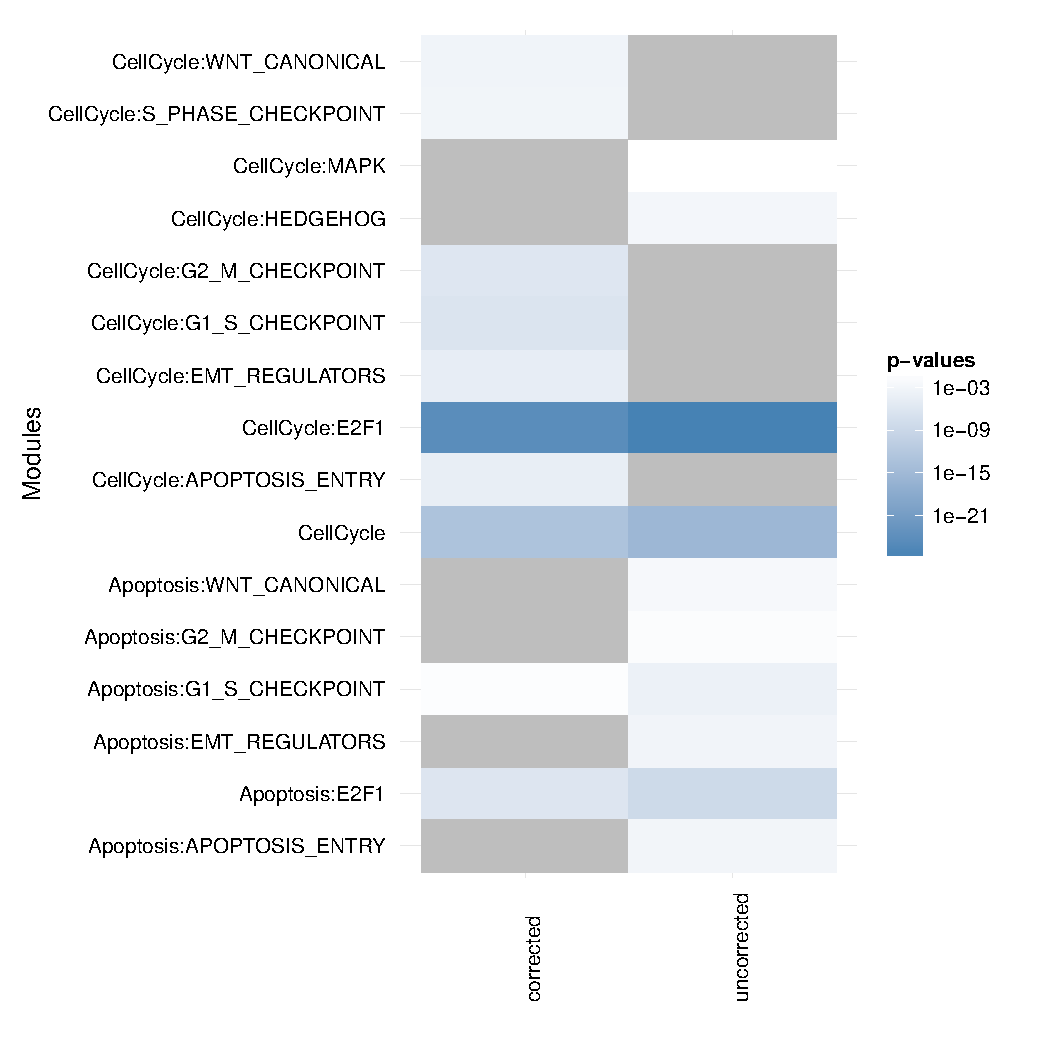
\includegraphics{figures/comparison_corrected_unc.pdf}
    \label{fig:heatm}

\end{figure}


\begin{figure}
	\caption{Representation of the enriched modules (first ten rows), either with either Bonferroni correction (left) or no correction (right). The modules are on the X axis and the p-values are on the Y axis.  }
	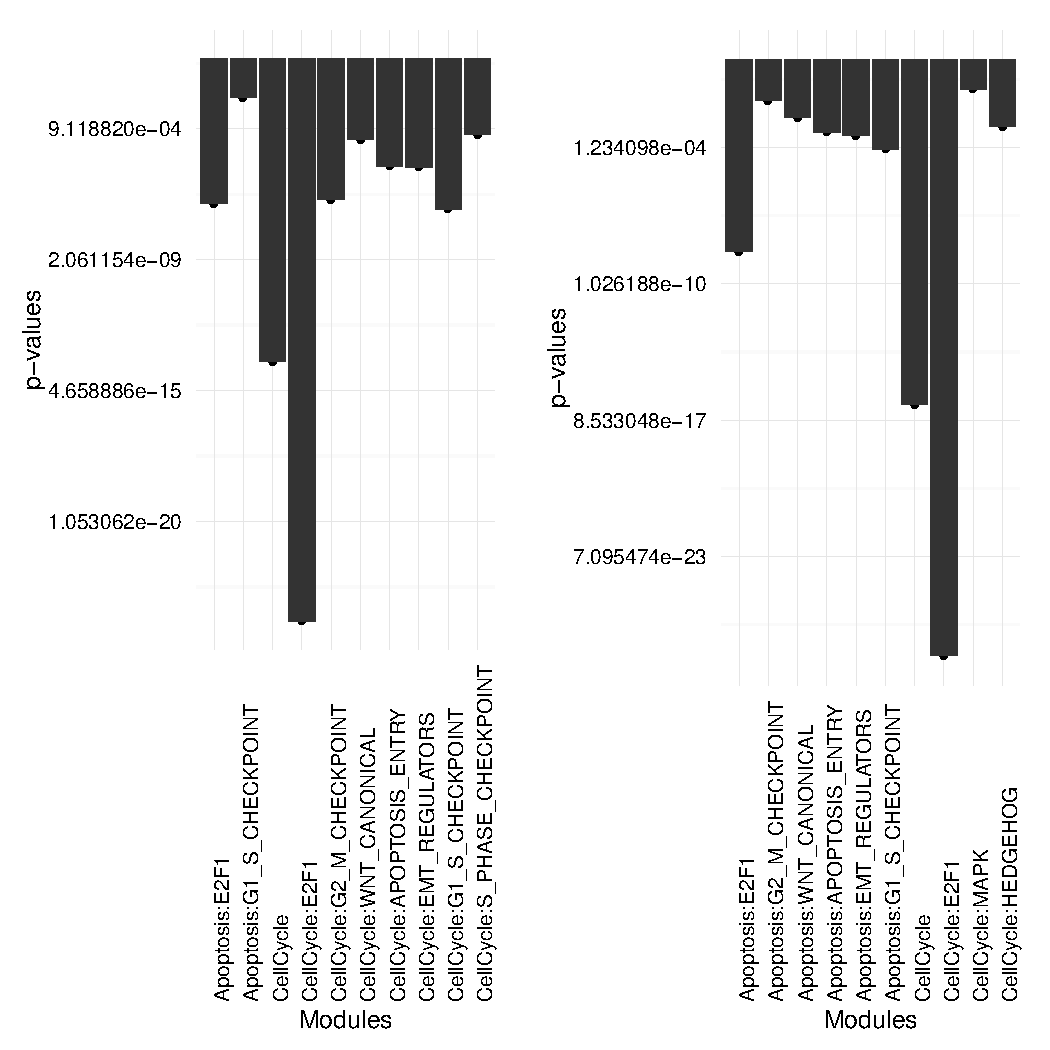
\includegraphics{figures/comparison_corrected_unc_bars.pdf}
	\label{fig:barp}

\end{figure}




\subsection{RNaviCell}

The NaviCell Web Service provides a server mode, which allows automating
visualization tasks and retrieving data from molecular maps via RESTful
(standard http/https) calls. Bindings to different programming languages are
provided in order to facilitate the development of data visualization workflows and
third-party applications \citep{bonnet2015navicell}. RNaviCell is the R binding
to the NaviCell Web Service. It is implemented as a standard R package, using
the R object-oriented framework known as Reference Classes \citep{hwR5}. Most
of the work done by the user using graphical point-and-click operations on the
NaviCell web interface are encoded as functions in the library encapsulating
http calls to the server with appropriate parameters and data. Calls to the
NaviCell server are performed using the library RCurl \citep{rcurl2015}, while
data encoding/decoding in JSON format is performed with the RJSONIO library
\citep{rjsonio2014}.

Once the RNaviCell library is installed and loaded, the first step is to create
a NaviCell object and launch the browser session. This will automatically create
a unique session ID with the NaviCell server. Once the session is established,
various functions can be called to send data to the web session, set graphical
options, visualize data on a map or get data from the map. There are 125
functions available in the current version of RNaviCell. All of them are
described with their different options in the RNaviCell documentation, and we
provide a tutorial on the GitHub repository wiki
(\url{https://github.com/sysbio-curie/RNaviCell/wiki/Tutorial}).  

In the simple example detailed below, we create a NaviCell session, then load
an expression data set from a local (tab-delimited) file. The data represent
gene expression measured in a prostate cancer cell line resistant to hormonal
treatment (agressive), and is taken from the Cell Line Encyclopedia project
\citep{barretina2012cancer}. We visualize the data values on the Cell Cycle map
(the default map), using heat maps. With this visualization mode, gene
expression values are represented as a color gradient (green to red) in
squares positioned next to the entities where the gene has been mapped (Figure~\ref{fig:du145}).      


\begin{figure}[!ht]
  \caption{Gene expression values from a prostate cancer cell line visualized
on the cell cycle map as heat map plots. The figure is a screenshot of the
NaviCell map browser, with the map set at the top (the less detailed) zoom
level. The essential phases of the cell cycle are indicated on the map
(G1/S/G2/M).} 
  \centering
  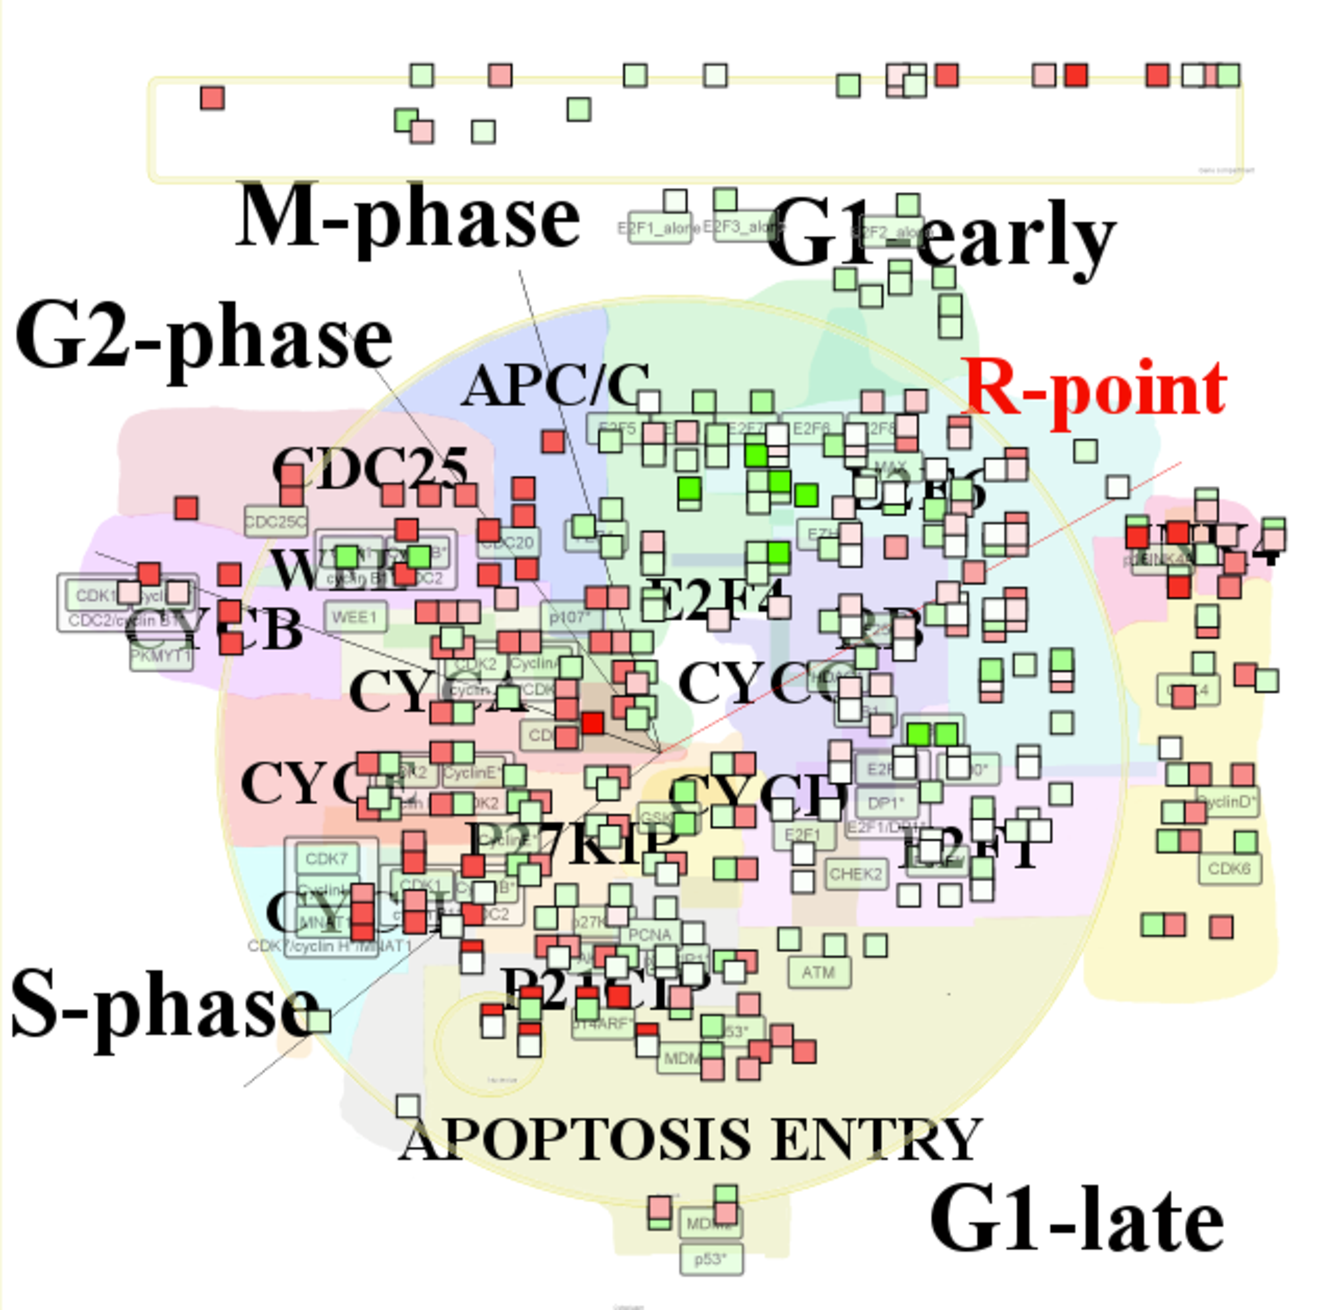
\includegraphics[width=0.8\textwidth]{figures/heatmap.pdf}
  \label{fig:du145}
\end{figure}



\begin{verbatim}
# a short RNaviCell script example

# load RNaviCell library

library(RNaviCell)

# create a NaviCell object and launch a server session
# this will automatically open a browser on the client 

navicell <- NaviCell()
navicell$launchBrowser()

# import a gene expression matrix and 
# send the data to the NaviCell server
# NB: the data_matrix object is a regular R matrix

data_matrix <- navicell$readDatatable('DU145_data.txt')
navicell$importDatatable("mRNA expression data", "DU145", data_matrix)

# set data set and sample for heat map representation

navicell$heatmapEditorSelectSample('0','data')
navicell$heatmapEditorSelectDatatable('0','DU145')
navicell$heatmapEditorApply()

\end{verbatim}

%navicell$launchBrowser()
\section[Examples]{Examples}

\subsection{Analysis of breast cancer expression data}
In a study published in 2008, Schmidt and colleagues analyzed gene expression
patterns of 200 breast cancer patients not treated by systemic therapy after
surgery using discovery approach to reveal additional prognostic motifs
\cite{schmidt2008humoral}. Estrogen receptor (ER) expression and proliferative
activity of breast carcinomas are well-known and described prognostic markers.
Patients with ER-positive carcinomas have a better prognosis than those with
ER-negative carcinomas, and rapidly proliferating carcinomas have an adverse
prognosis. Knowledge about the molecular mechanisms involved in the
processes of estrogen-dependent tumor growth and proliferative activity has led
to the successful development of therapeutic concepts, such as  antiendocrine and
cytotoxic chemotherapy. 

The dataset corresponding to this study is available as a
Bioconductor package. The code shown below is creating a list of differentially
expressed genes 

\begin{verbatim}

library(breastCancerMAINZ)
library(Biobase)
library(limma)
library(ACSNMineR)
library(hgu133a.db)
library(RNaviCell)

data(mainz)
eset <- exprs(mainz)
pdat <- pData(mainz)
design <- model.matrix(~factor(pdat$er == '1'))
lmFit(eset, design) -> fit
eBayes(fit) -> ebayes
toptable(ebayes, coef=2,n=25000)->tt
#which(abs(tt$logFC) >=1 & tt$adj < 0.05) -> sel
which(tt$adj < 0.05) -> sel
rownames(tt[sel,]) -> probe_list
mget(probe_list, env=hgu133aSYMBOL) -> slist
slist <- as.character(slist)

enrichment(slist) -> res

#apply(eset[probe_list,pdat$er == 1],1,mean)->er_plus_mean
#apply(eset[probe_list,pdat$er == 0],1,mean)->er_minus_mean
#cbind(er_plus_mean, er_minus_mean)-> data_er
#rownames(data_er) <- slist

#n$map_url <- "http://acsn.curie.fr/navicell/maps/apoptosis/master/index.php"
#n$importDatatable("mRNA expression data", "exp", data_er)

apply(eset[probe_list,pdat$er == 0],1,mean) -> er_minus_mean
names(er_minus_mean) <- slist
er_minus_mean <- as.matrix(er_minus_mean)
colnames(er_minus_mean) <- c('exp')


n <- NaviCell()
n$proxy_url <- "https://acsn.curie.fr/cgi-bin/nv_proxy.php"
n$map_url <- "https://acsn.curie.fr/navicell/maps/acsn/master/index.php"

n$launchBrowser()
n$importDatatable("mRNA expression data", "GBM_exp", er_minus_mean)
n$heatmapEditorSelectSample('0','exp')
n$heatmapEditorSelectDatatable('0','GBM_exp')
n$heatmapEditorApply()

# analysis mtsig signature file

#mt <- format_from_gmt('/Users/eric/Downloads/c2.cp.v5.0.symbols.gmt')
#unique(slist)->l
#> length(l)
#[1] 5179
#> head(l)
#[1] "ESR1"   "CA12"   "GATA3"  "TBC1D9" "FOXA1"  "IL6ST" 
#> enrichment(l, maps=mt)

\end{verbatim}



%\bibliographystyle{jss}
\bibliography{biblio}

\end{document}
